\documentclass[a4paper]{article}
\usepackage[utf8]{inputenc}

% Add support for text columns
\usepackage{multicol}
\setlength{\columnsep}{1cm}

% Bibliography
\usepackage{biblatex}
\addbibresource{references.bib}

% Figures and Subfigures
\usepackage{graphicx}
\usepackage{float}
\usepackage{subcaption} % Subfigures

% Utilize the full page
\usepackage[margin=1.2cm]{geometry}
\addtolength{\topmargin}{-1.2cm}

\title{Computer Graphics (1TD388) \\ Uppsala University -- Spring 2016 \\ Particle System Project Report}
\author{Lucas Arnström}
\date{\today}

\begin{document}

\maketitle

\begin{figure}[htbp]
    \centering
    \begin{subfigure}[ht]{0.22\textwidth}
        
\includegraphics[width=\textwidth]{figures/explosion.png}
        \caption{Explosion}
        \label{fig:simulations_explosion}
    \end{subfigure}
    \begin{subfigure}[ht]{0.22\textwidth}
        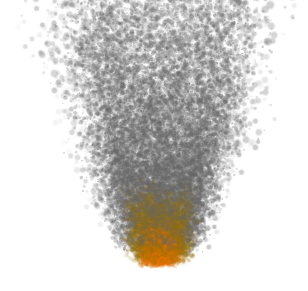
\includegraphics[width=\textwidth]{figures/fire.png}
        \caption{Fire}
        \label{fig:simulations_fire}
    \end{subfigure}
    \begin{subfigure}[ht]{0.22\textwidth}
        
\includegraphics[width=\textwidth]{figures/tornado.png}
        \caption{Tornado}
        \label{fig:simulations_tornado}
    \end{subfigure}
    \begin{subfigure}[ht]{0.22\textwidth}
        
\includegraphics[width=\textwidth]{figures/water.png}
        \caption{Fountain}
        \label{fig:simulations_fountain}
    \end{subfigure}

    \caption{Screenshots of the four different particle simulations produced by the program.}
    \label{fig:simulations}
\end{figure}

\begin{multicols*}{2}
\section{Abstract}

\section{My approach}

\section{Conclusion}

\printbibliography
\end{multicols*}

\end{document}
